
\section{Applications}


\begin{frame}{Protobuf}

\end{frame}

\begin{frame}{Cluster estimation}

%unsigned int cluster_estimate();

%$\hat{k} = \argmin_k \left\lVert D^{(k)} - \bar D \right\rVert_F^2 = \argmin_k \sum_{i,j} \left( D^{(k)}_{ij} - \bar{D}_{ij} \right)^2.
%$

\end{frame}

\begin{frame}{Density estimation}

%void eval_density(const std::vector<double> grid);

\begin{equation}
	\begin{aligned}
	\hat f^{(k)}(x) \ = \ \sum_j \frac{n^{(k)}_j}{M+n} f\left(x | \phi^{(k)}_j\right) \ + \ \frac{M}{M+n} m(x)
	\end{aligned}
\end{equation}

\begin{equation}
	\begin{aligned}
		\hat m(x) = \frac{1}{m} \sum_{h=0}^{m-1}  f\left(x | \phi_h\right)
	\end{aligned}
\end{equation}


$ \hat f(x) = \frac{1}{K} \sum_k \hat f^{(k)}(x) $

\end{frame}

\section{Results}


\begin{frame}{Auxiliary parameters}

\begin{center}
		%\texttt{a}
		\includegraphics[scale=0.5]{etc/dens_withmM10.pdf}
	\end{center}
\end{frame}


\begin{frame}{Oscillations}
\begin{figure}[h]
	\centering
	\begin{minipage}{0.5\textwidth}
		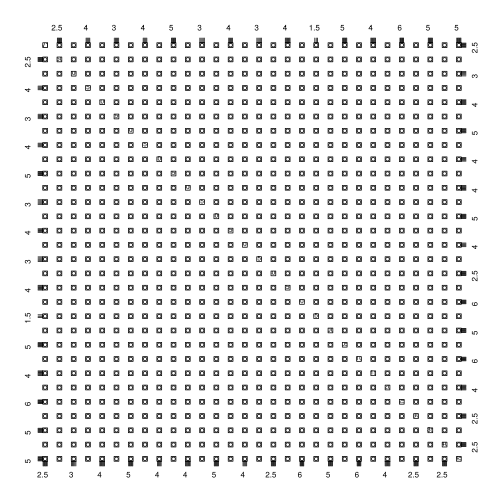
\includegraphics[scale=0.35]{etc/cardinalities_thinned.pdf}
	\end{minipage}%
	\begin{minipage}{0.5\textwidth}
		\includegraphics[scale=0.35]{etc/densities_iters.pdf}
	\end{minipage}
\end{figure}

\end{frame}

\begin{frame}{Total mass}

\begin{center}
		%\texttt{}
		\includegraphics[scale=0.35]{etc/num_clust_M.pdf}
	\end{center}


\begin{center}
		%\texttt{a}
		\includegraphics[scale=0.35]{etc/dens_withMm3.pdf}
	\end{center}
\end{frame}



\begin{frame}{Auxiliary parameters}

\begin{center}
		%\texttt{a}
		\includegraphics[scale=0.5]{etc/dens_withmM10.pdf}
	\end{center}
\end{frame}


\begin{frame}{Density components}

\begin{center}
		%\texttt{}
		\includegraphics[scale=0.35]{etc/componentsM025m3_best.pdf}
	\end{center}


\begin{center}
		%\texttt{a}
		\includegraphics[scale=0.35]{etc/barplotM1m3.pdf}
	\end{center}
\end{frame}



\begin{frame}{\texttt{Neal2} vs \texttt{Neal8}}

\begin{center}
		%\texttt{a}
		\includegraphics[scale=0.5]{etc/neal2_M10.pdf}
	\end{center}
	
\end{frame}
